%Matteo Kumar - Leonard Schatt
% Fortgeschrittenes Physikalisches Praktikum

\clearpage
\section{Fitten der Shockley-Gleichung}
\label{chapter:fitten}

Aus den Daten wurde mithilfe einens MatLab-Programmes ref die Parameter, welche in der Shockley-Gleichung vorkommen ref gefittet. Dabei wird beachtet, 
dass bei der CIS-Zelle einen Reihenschaltung von 11 kleinen Solarmodulen vorhanden ist. Daher wird die Spannung durch 11 geteilt. Leider erhält man 
trotzdem sehr fragwürdige Parameter, beispielsweise unrealistisch hohe Temperaturen als Umgebungsbedingungen hatten. Diese sind aber ausgeschlossen, 
da die Temperatur als Referenz gemessen wurde.
Interessant ist vorallem, dass sich mit dem Programm vor allem die Multi- und MonoSi besser mitder Shockley-Gleichung gefittet werden, als 
die CIS Solarzelle, was aber auch gut an der fehlerhaften Anwendung des Programmes oder dem Programm selbst.

\subsection{CIS-Solarmodul}

Nach dem fitten mit dem oben erwähnten Programm erhält man folgende Abbildungen und Parameter.

\begin{figure}[ht]
    \centering
    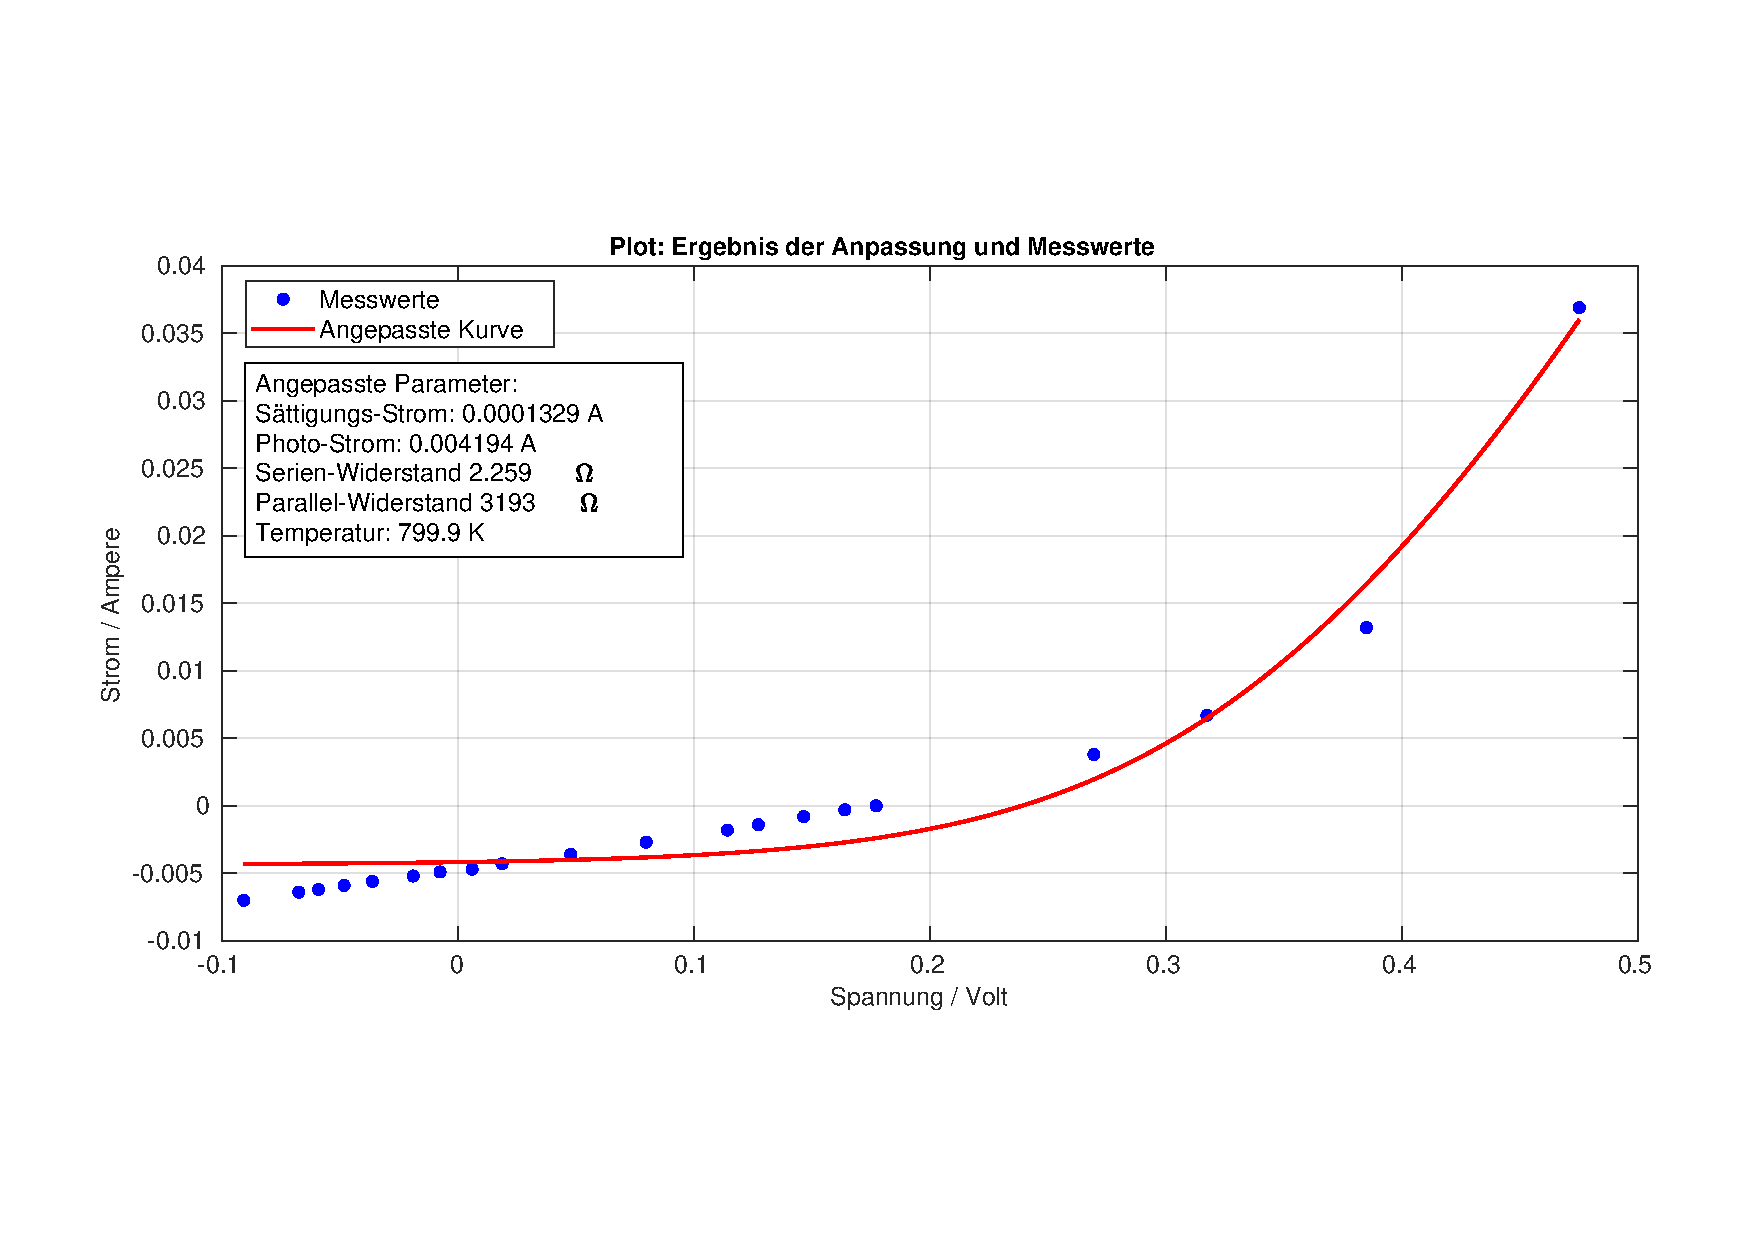
\includegraphics[width = \linewidth]{Bilder/CIS130Plot.pdf}
    \caption{Gefittete Shockley-Gleichung an das CIS-Modul bei 130V Trafospannung}
    
\end{figure}

\begin{figure}[ht]
    \centering
    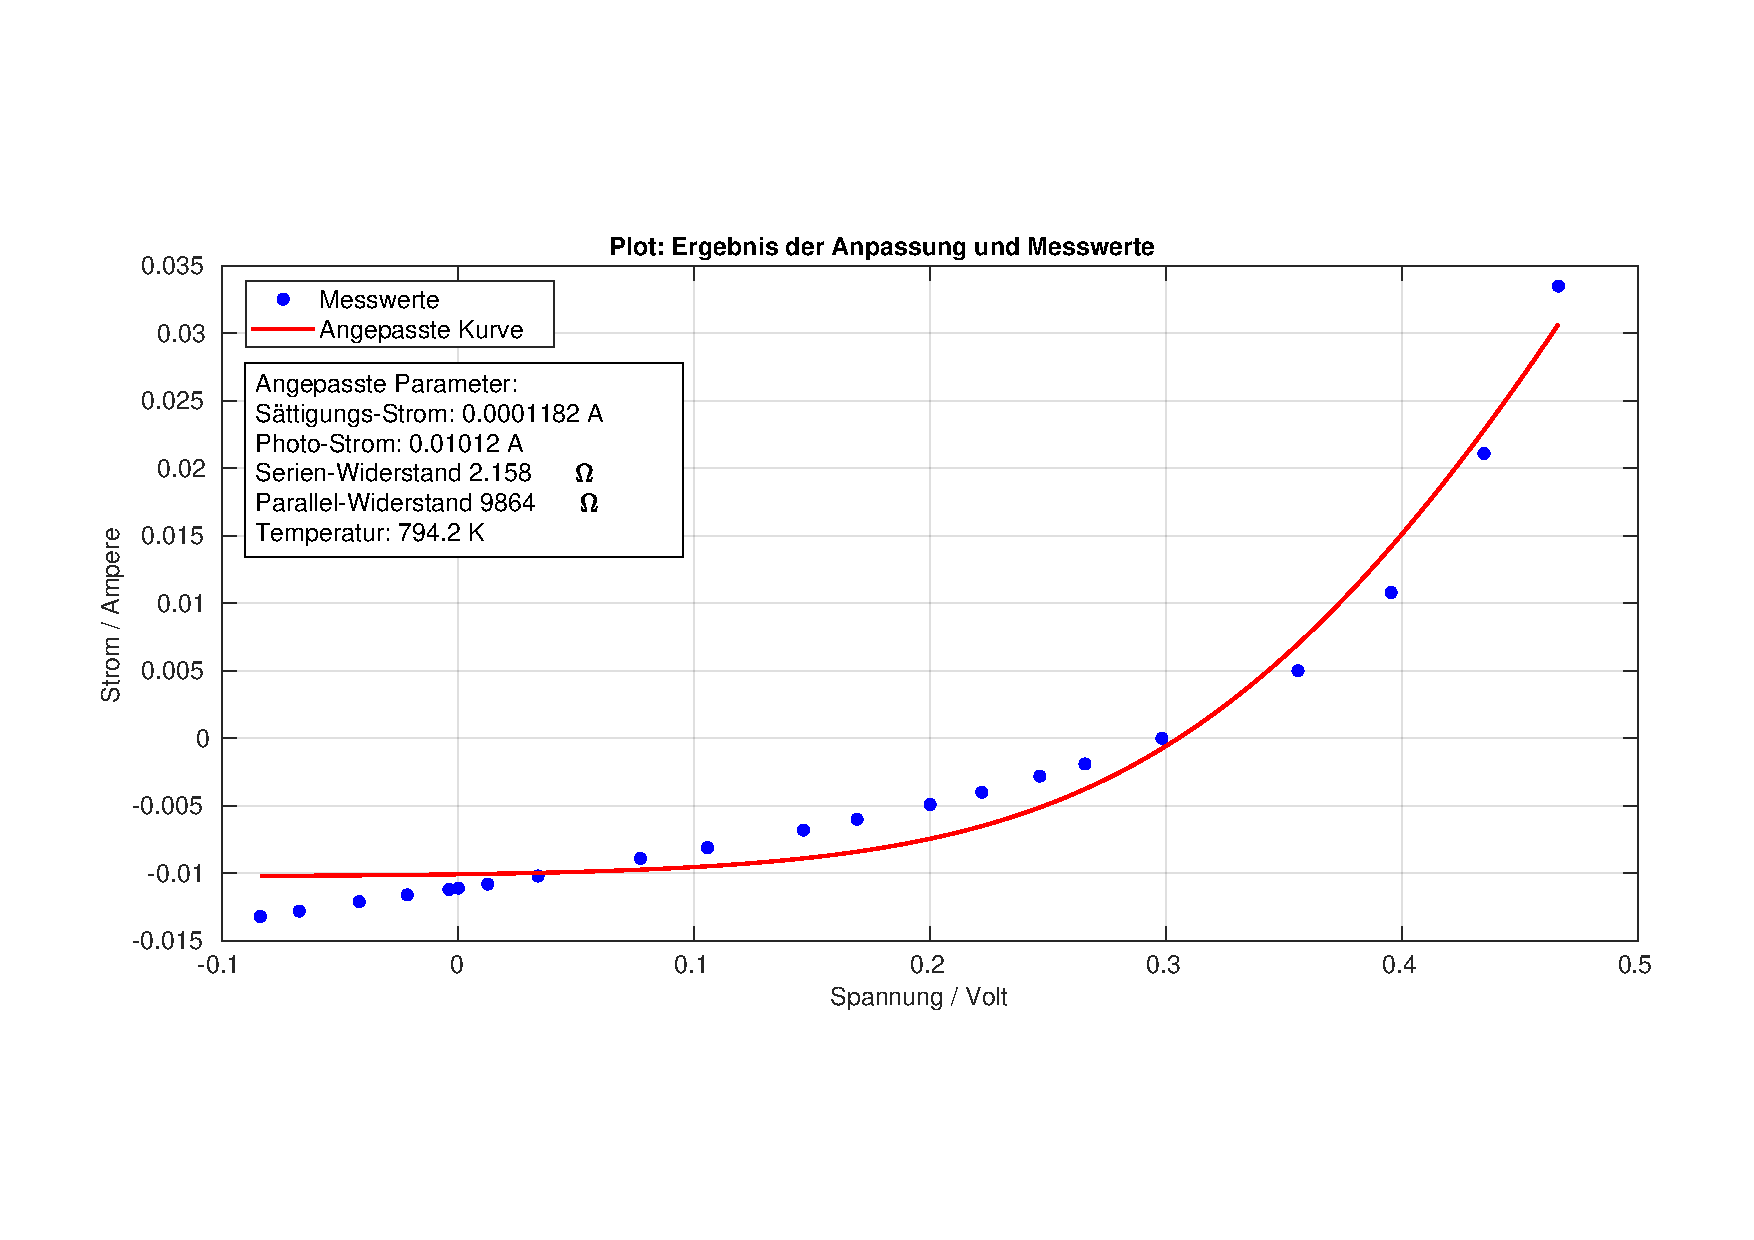
\includegraphics[width = \linewidth]{Bilder/CIS180Plot.pdf}
    \caption{Gefittete Shockley-Gleichung an das CIS-Modul bei 180V Trafospannung}    
\end{figure}

\begin{figure}[ht]
    \centering
    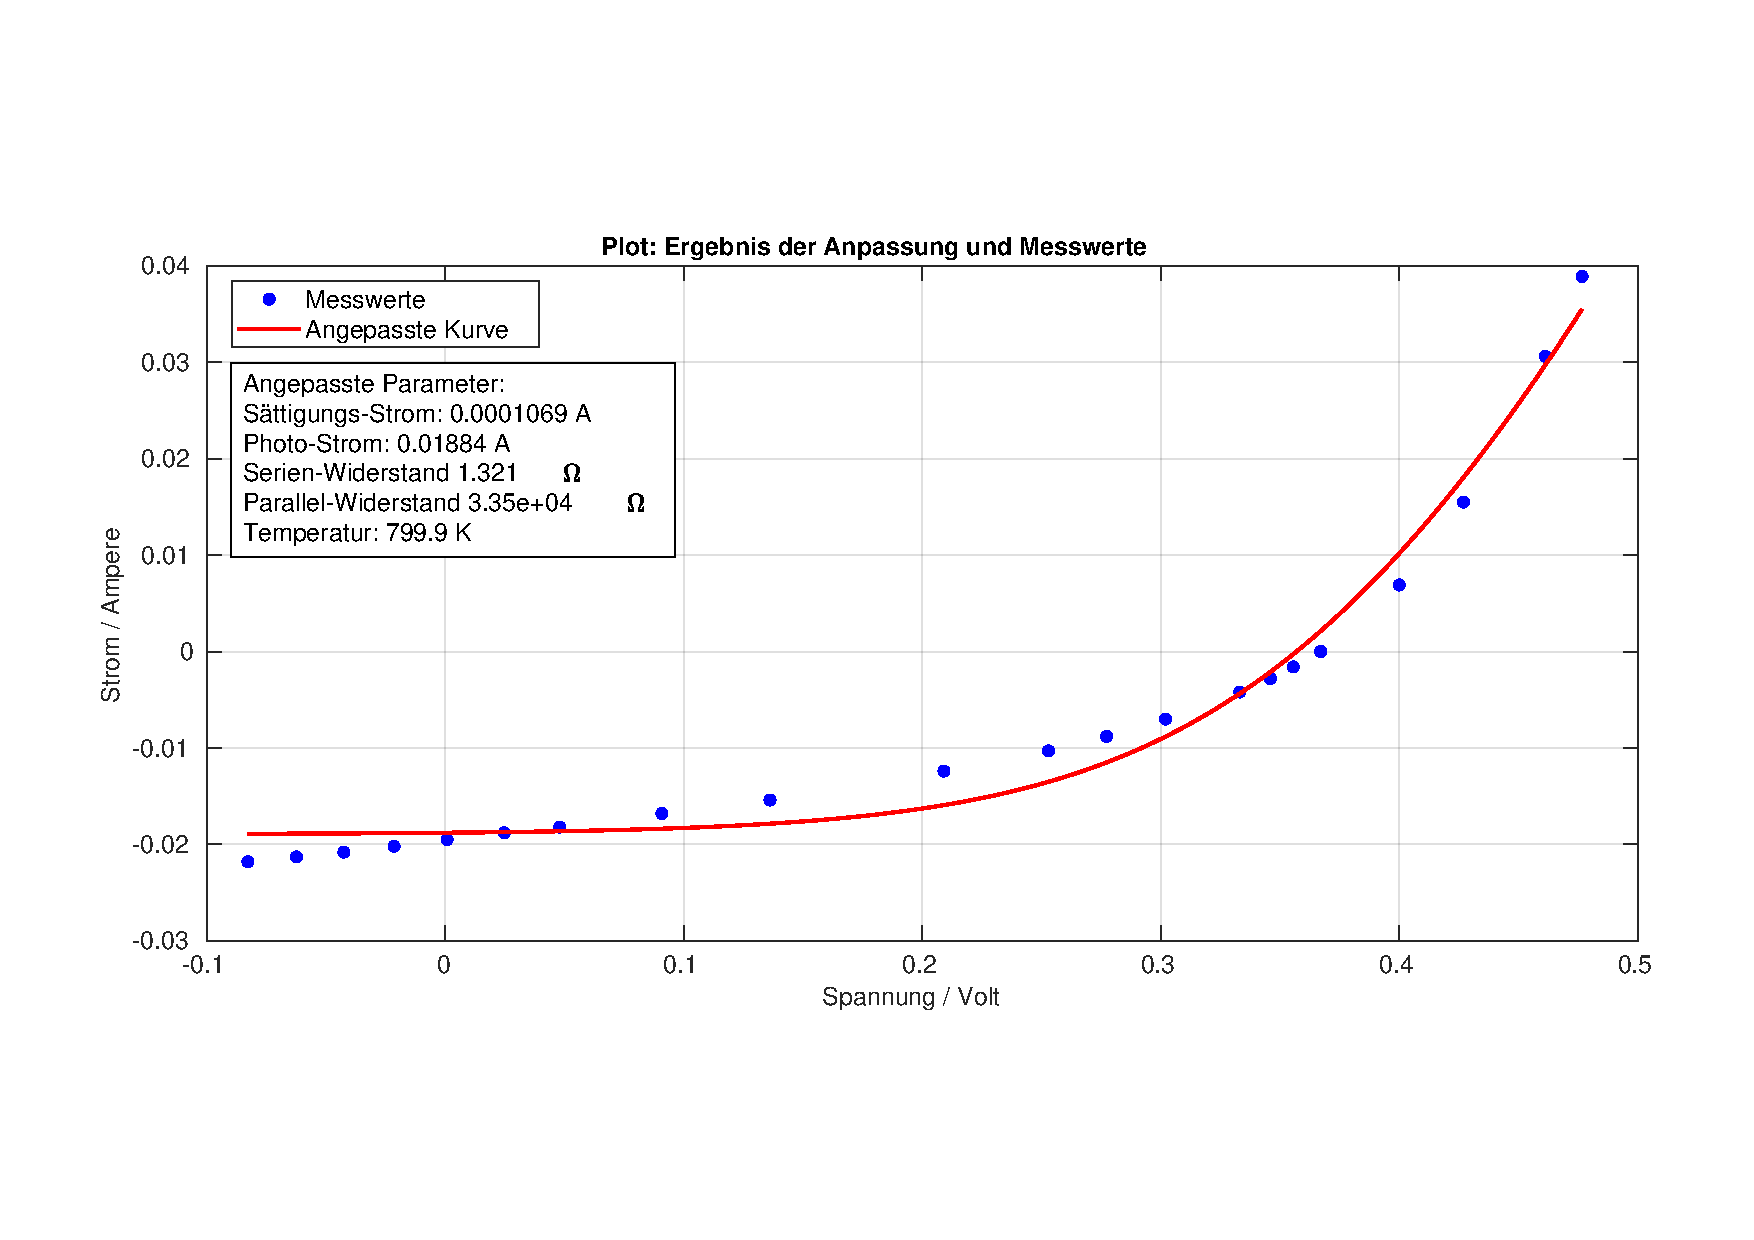
\includegraphics[width = \linewidth]{Bilder/CIS230Plot.pdf}
    \caption{Gefittete Shockley-Gleichung an das CIS-Modul bei 230V Trafospannung}
\end{figure}

Dabei fällt vor allem die ungewöhnlich hohe Temperatur, wie auch die riesigen Reihen- und Parallel-Widerstände auf. 
Da die Werte sehr unrealistisch erscheinen, ist darauf zu schließen, dass sich irgendwo ein Fehler eingschlichen hat, 
den wir leider auch bei genauer Betrachtung nicht ermitteln konnten.

\begin{figure}[ht]
    \centering
    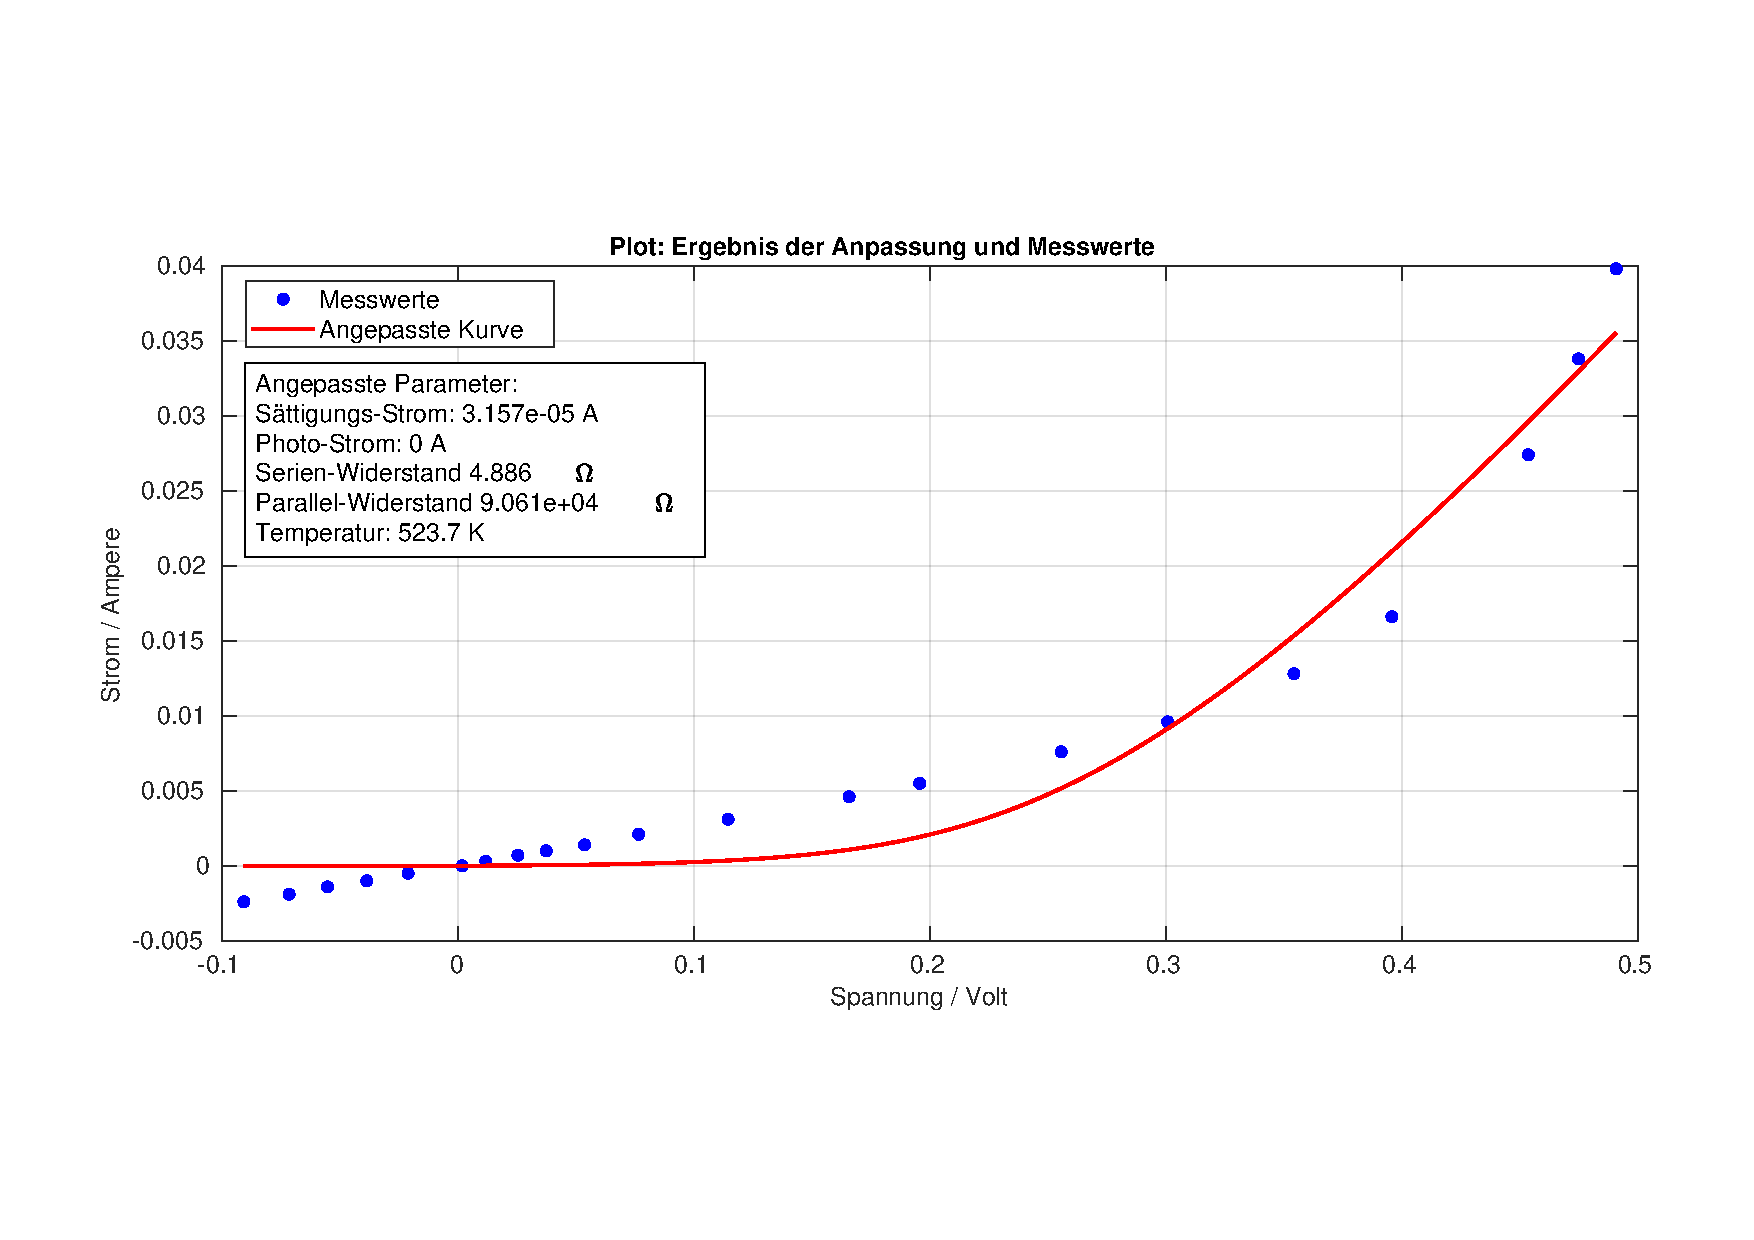
\includegraphics[width = \linewidth]{Bilder/CISDunkelPlot.pdf}
    \caption{Gefittete Schockley-Gleichung an Dunkelmessung der CIS-Zelle}
\end{figure}

\clearpage

\subsection{Mono- und MultiSi-Zellen}

Auch Mono- und MultiSi-Module wurden versucht mit dem Programm zu fitten. Dabei funktionierte das hier sichtlich besser.

\begin{figure}[ht]
    \centering
    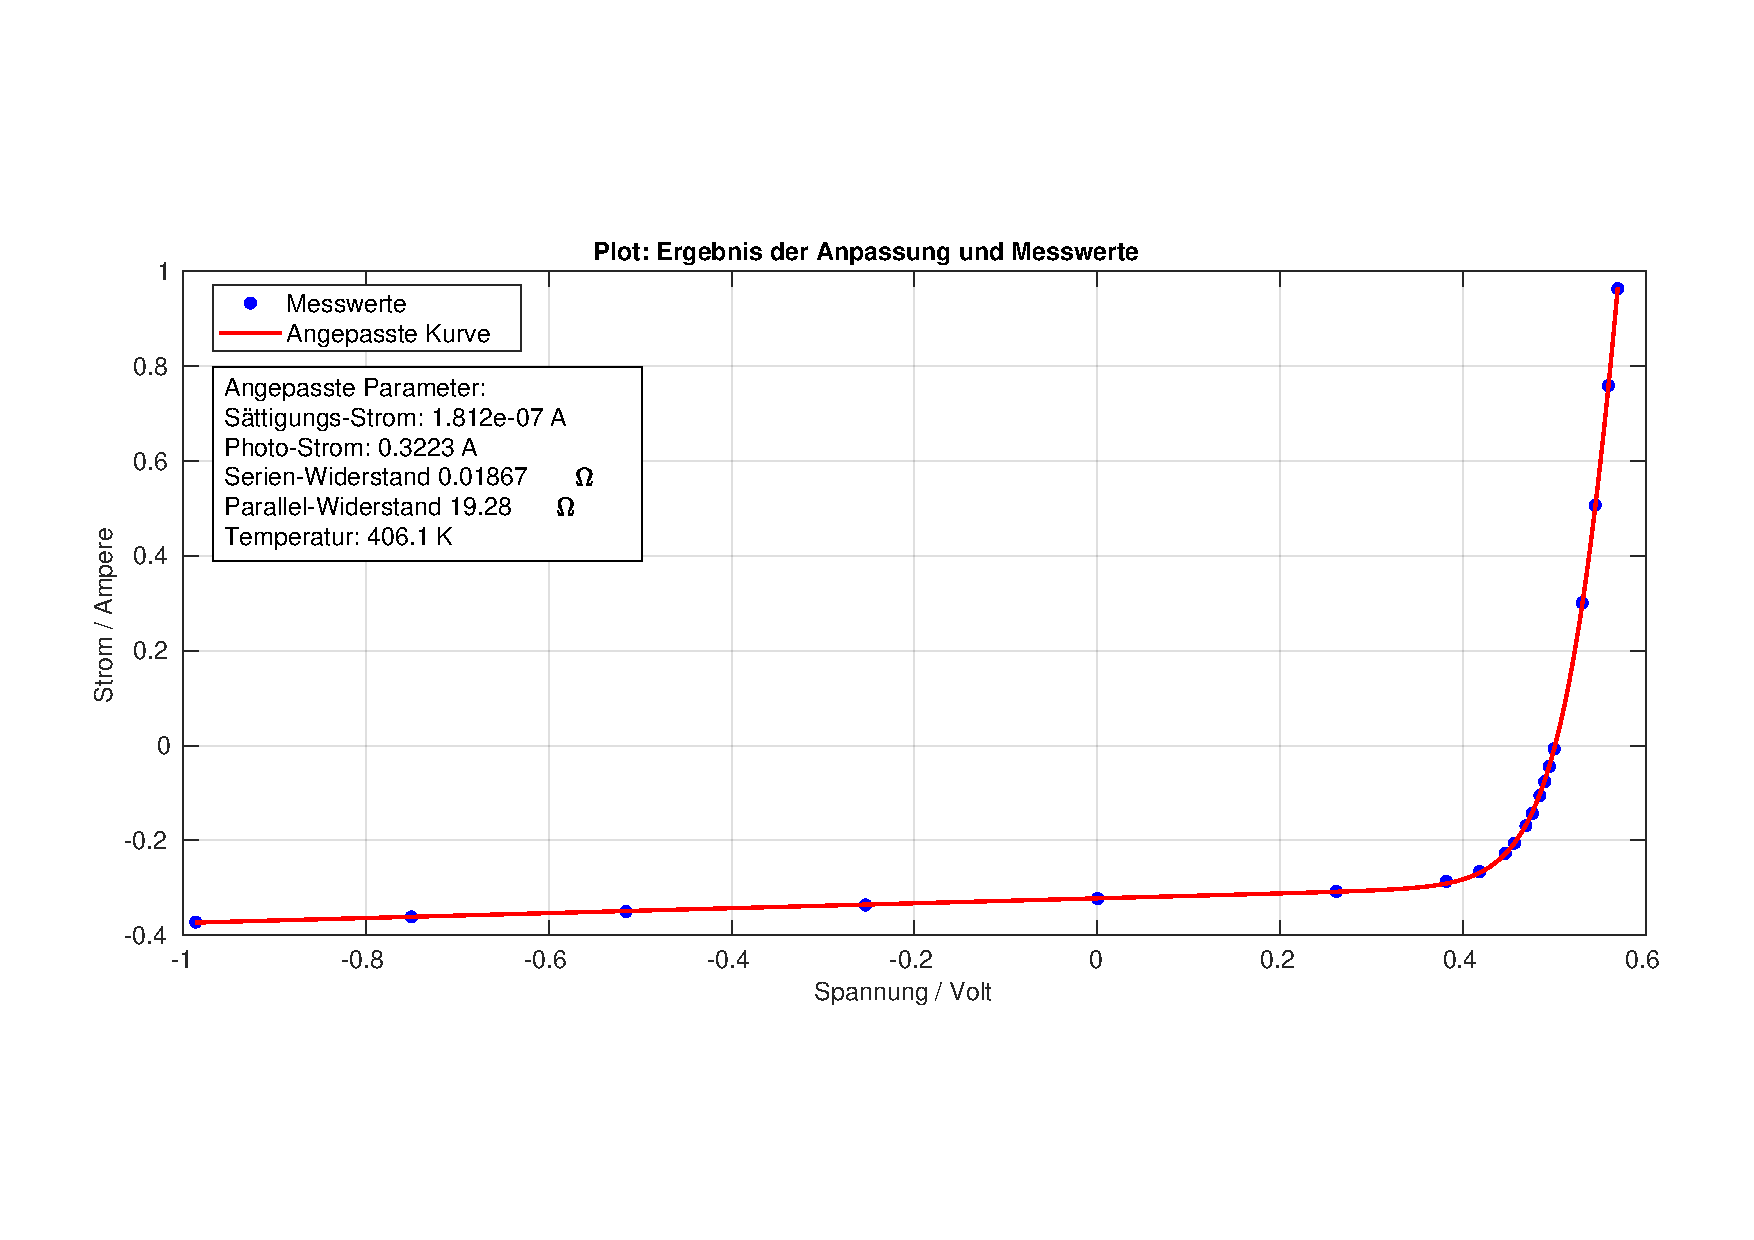
\includegraphics[width = \linewidth]{Bilder/SiMono130Plot.pdf}
    \caption{Gefittete Schockley-Gleichung an das Mono-Si-Modul bei 130V}
\end{figure}

\begin{figure}[ht]
    \centering
    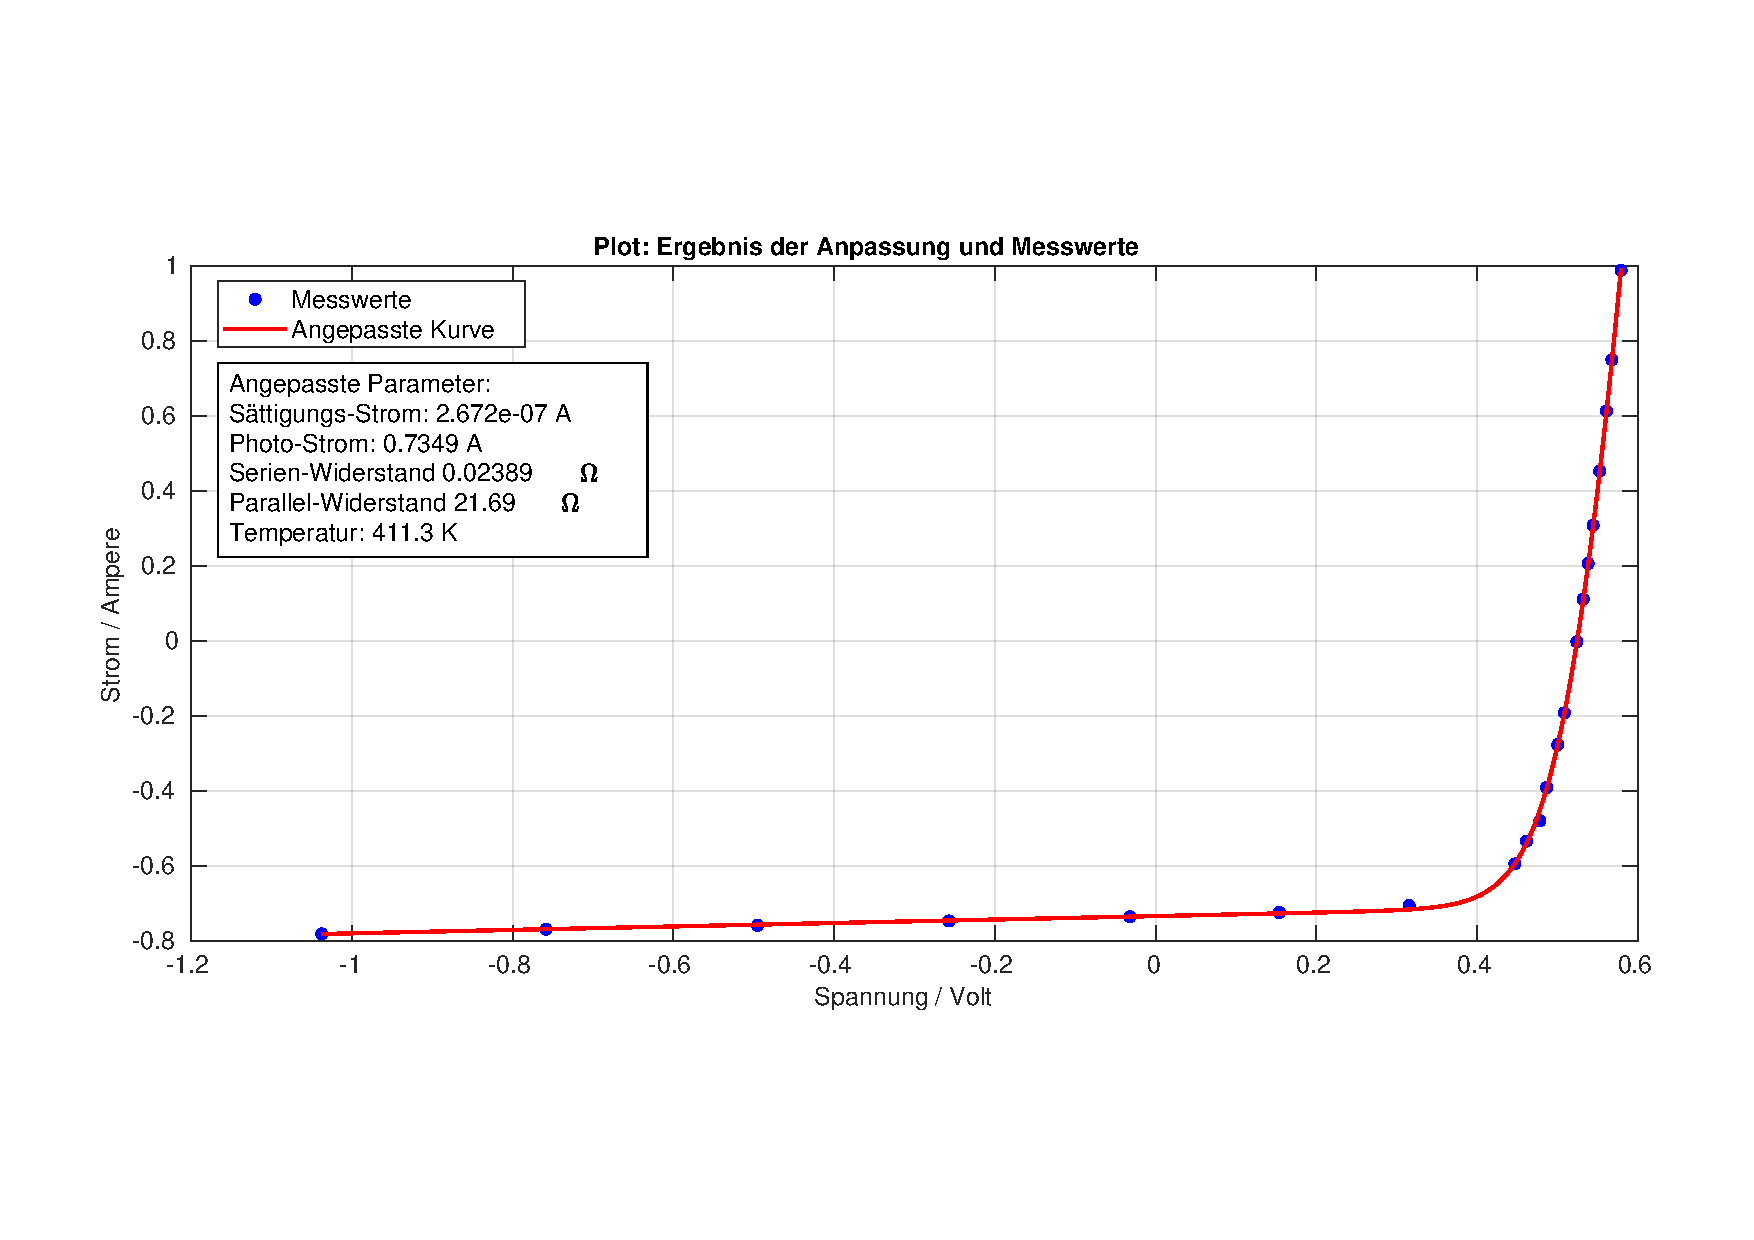
\includegraphics[width = \linewidth]{Bilder/SiMono180Plot.pdf}
    \caption{Gefittete Schockley-Gleichung an das Mono-Si-Modul bei 180V}
\end{figure}


\begin{figure}[ht]
    \centering
    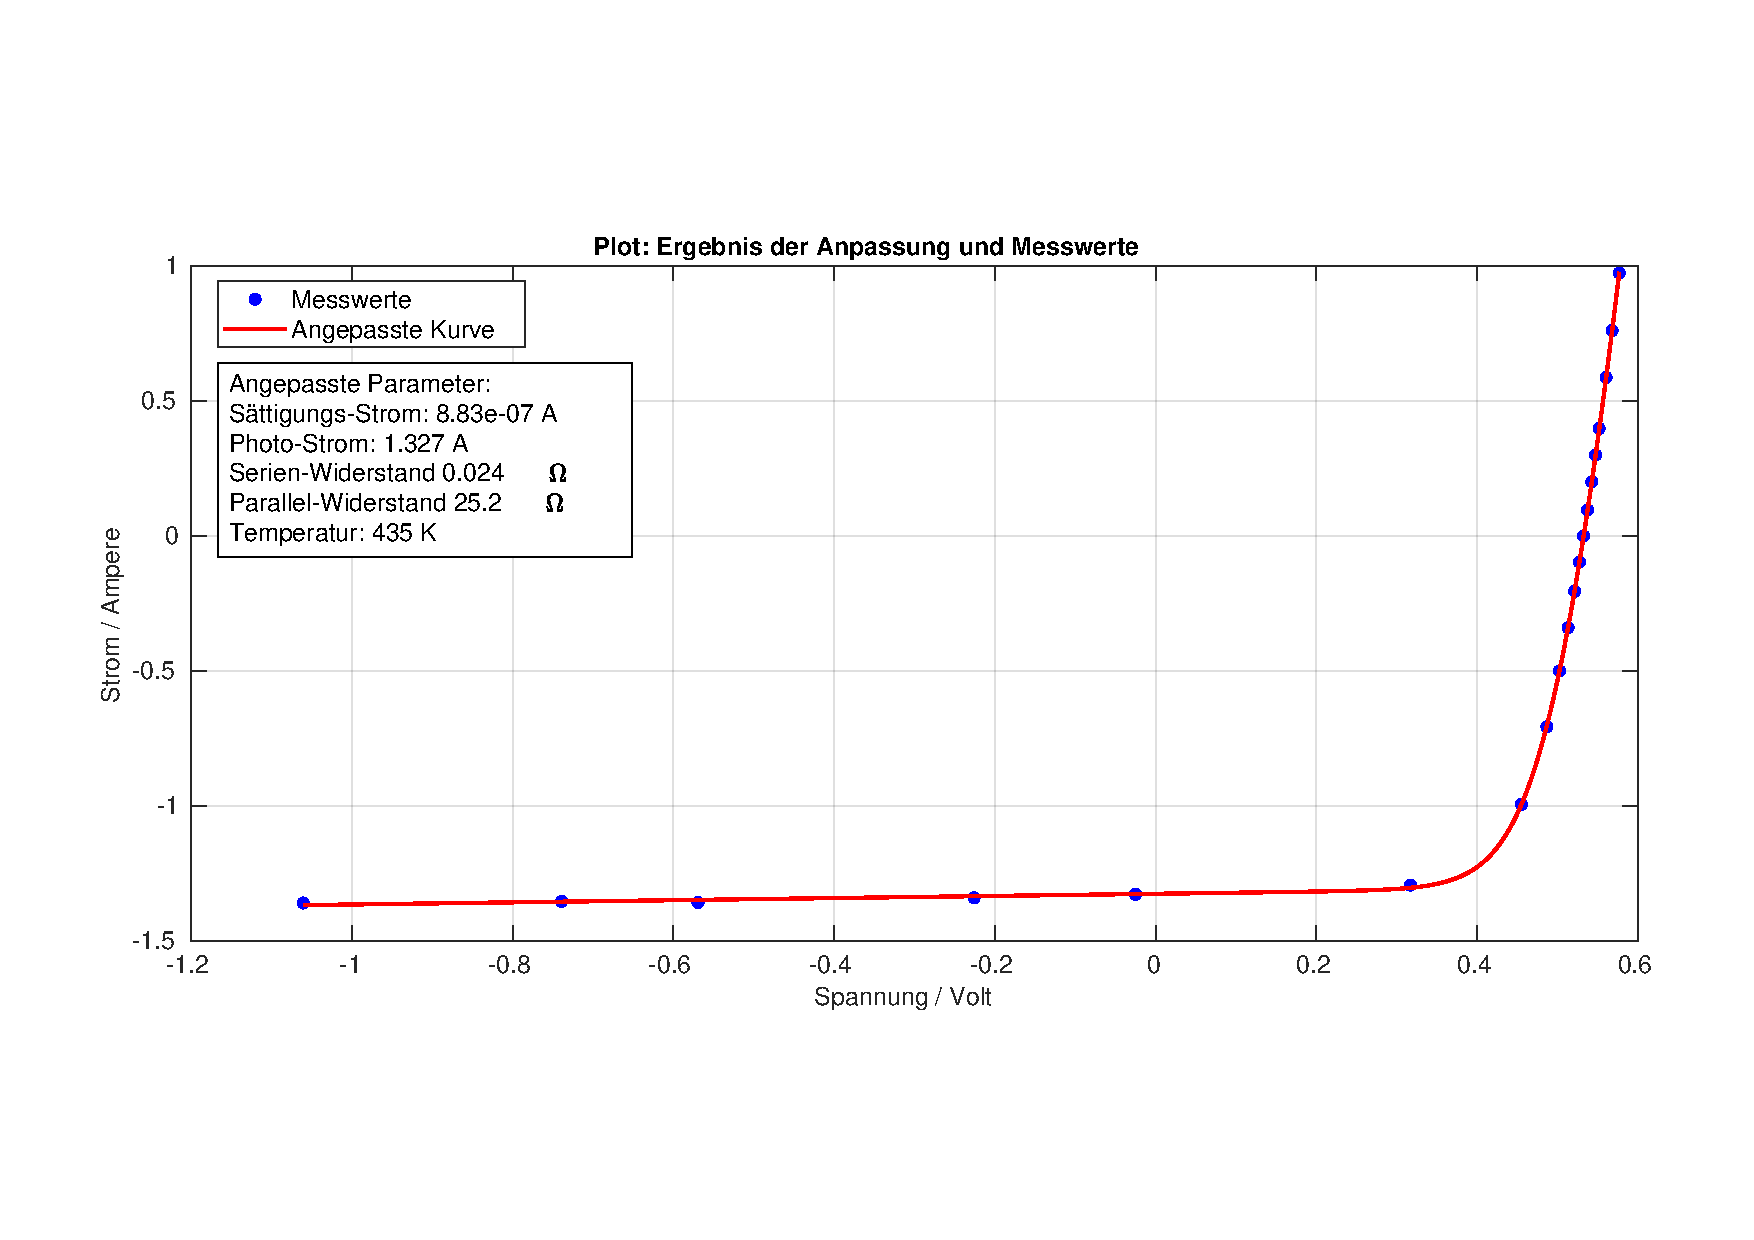
\includegraphics[width = \linewidth]{Bilder/SiMono230Plot.pdf}
    \caption{Gefittete Schockley-Gleichung an das Mono-Si-Modul bei 230V}
\end{figure}


Dabei ist, wie erwartet, der Photostrom $I_{Ph}$ bei steigender Helligkeit immer stärker. Die restlich Grafiken befinden sich im Anhang. Bei 
allen ist schön das "nach unten verschieben" bei höherer Lichtleistung beobachtbar. \\
Die Füllfaktoren $FF$ und Strom und Spannung am $MPP$ ergeben sich nach grafischer Auswertung wie folgt:\\
\begin{table}[h]
    \centering
    \begin{tabular}{l|c|c|r}
        & Strom am $MPP$ (A) & Spannung am $MPP$ (V) & $FF$ \\
        \toprule
        SiMono bei 130V & 0.405 & -0.27 & 0.69 \\
        SiMono bei 180V & 0.416 &-0.66 & 0.71 \\
        SiMono bei 230V & 0.412 & -1.19 & 0.69\\
        \midrule
        SiMulti bei 130V & 0.398 & -0.25 & 0.70 \\
        SiMulti bei 180V & 0.414 & -0.55 & 0.71 \\
        SiMulti bei 230V & 0.435 & -1.05 & 0.74\\
        \midrule
        CIS bei 130V & 0.151 &  -0.0029 & 0.44 \\
        CIS bei 180V & 0.202 & -0.0073 & 0.48 \\
        CIS bei 230V & 0.238 & -0.0144 & 0.51\\
    \end{tabular}
\end{table}

Dabei ist auffällig, dass am $MPP$ die Spannungswerte immer nahezu identisch sind. Die Stromwerte steigen aber eindeutig. Außerdem ist der 
niedrige Füllfaktor bei de, CIS-Modul auffällig. Daraus würde man ein langsames Ansteigen der Kurve vermuten, welches man dann im Bild auch beobachten kann. 
Die CIS-Zelle ist somit am weitesten von einer idealen Solarzelle entfernt, da sie den langsamen ansteig hat. Das erklärt auch, warum beim fitten die 
hohe Temperatur vorgeschlagen wird, da diese zu einem langsameren Anstieg der U_I_Kennlinie führt. Insgesamt beschreibt das Ersatzschaltbild 
die CIS-Zelle möglicherweise nicht gut.

\clearpage

\subsection{Idealitätsfaktor}

Der Idealitätsfaktor $n$ ist ein Faktor, der beschreibt, wie gut sich der Halbleiter, beziehungsweise hier der pn-Übergang durch das Bändermodell 
darstellen lässt. Dabei kann man diesen relativ einfach aus der Shockley-Gleichung gewinnen.

\begin{equation}
    n =  \frac{qU}{kT} \frac{1}{\ln{(\frac{I_{Ph}+\frac{R_S I -U}{R_P}+I}{I_0}+1)}}
    \label{Ideal1}
\end{equation}

Bei der Gleichung ist $I_0$ der Sättigungsstrom, $I_PH$ der Fotostrom, $U$ die Spannung, $R_{S}$ und $R_{P}$ der Reihen- und Parallelwiderstand.\\
Gleichung \ref{Ideal1} kann man nochmal vereinfachen, indem man an der Stelle (U,I)= ($U_{OC}$,0A) einsetzt.

\begin{equation}
    n =  \frac{qU}{kT} \frac{1}{\ln{(\frac{I_{Ph}-\frac{U_{OC}}{R_P}}{I_0}+1)}}
    \label{Ideal2}
\end{equation}

Setzt man die in Kapitel \ref{chapter:fitten} erhaltenen Werte ein, so erhalt man als Idealitätsfaktoren die folgenden Werte.

\begin{table}[h]
    \centering
    \begin{tabular}{l|r}
        MonoSi-Modul & $n$ = 1.004\\
        MultiSi-Modul & $n$ = 1.004\\
        CIS-Modul & $n$ = 1.003\\
    \end{tabular}
    \caption{Idealitätsfaktoren der Solar-Module }
\end{table}

Wie bei den obigen Werten ist es schwer überhaupt Fehler anzugeben, da die einzelnen Parameter aus der Shockley-Gleichung 
schwer im Fehler abzuschätzen sind. Eine Unsicherheit von 10\% wäre jedoch sichern nicht vermessen.\
Im Gesamten kann man sagen, dass die obigen Werte durchaus realistisch erscheinen. Eine 
Diode sollte einen Idealitätsfaktor zwischen 1-2 haben. Hier liegen wir schon nah an 1, dass 
heißt, dass sich die Solar-Module sehr gut durch das Bändermodell beschreiben lassen.


\subsection{Wirkungsgrad}

Eine spannende Frage ist nun, wie es sich mit dem Wirkungsgrad in Abhängigkeit von der Beleuchtungsstärke verhält. 
Dabei berechnet man die Lichtintensität aus den Referenzmessungen mit der kalibrierten Solarzelle. Mithilfe dieser 
bestimmt man die Lichtleitung $P_L$. Der Wirkungsgrad $\eta$ ergibt sich dann wie im theoretischen Teil beschrieben. 

\begin{figure}[h]
    \centering
    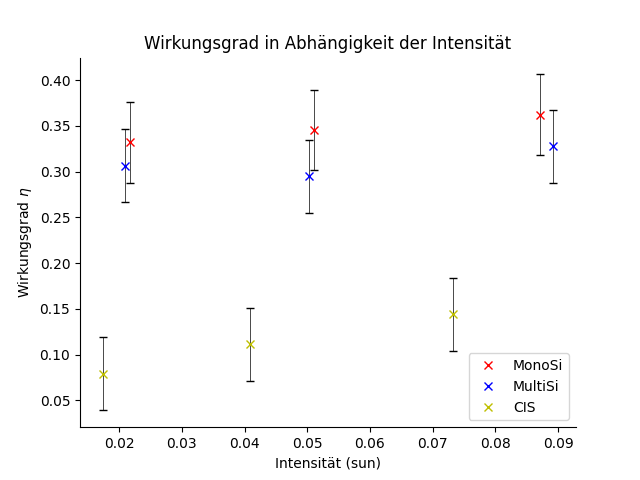
\includegraphics[width = \linewidth]{Bilder/PlotWirkungsgradInt.png}
\end{figure}

Dabei kann man einen ganzlichten Trend zu einem besseren Wirkungsgrad bei höheren Frequenzen sehen. Dies ist vermutlich ein 
temperaturbedingter Effekt, da die Module bei höheren Intensitäten deutlich wärmer wurden. Desweiten sieht man schön den Unterschied 
im Wirkungsgrad zwischen der MonoSi- und der MultiSi-Solarzelle. Die monokristalline Solarzelle hat, wie erwartet, einen etwas höheren 
Wirkungsgrad. Dabei sind beide etwas zu hoch angesiedelt. 
Die CIS-Zelle hingegen hat einen deutlich zu niedrigen Wirkungsgrad, was vermutlich auf einen Rechenfehler zurück zu führen ist.\

Auffällig ist dabei noch, dass die Spannung $U_{OC}$ relativ konstant bleibt, der Photostrom hingenen linear mit der Beleuchtungsstärke zunimmt. 
Im Gesamten bleibt die Form der Kurve jedoch ähnlich, was man auch an konstanten Füllfaktoren sieht. Die Grafiken dazu im Anhang.


\subsection{Extrapolieren der Photostroms}

Der Photostrom $I_{Ph}$ wird bis 1sun extrapoliert. Dabei wird ein linearer Zusammenhang angenommen, da eine Zunahme der Lichtintensität direkt proportional zu der 
Anzahl der Photonen ist. Der Photostrom hängt von der Anzahl der Elektronen ab, die durch den photoelektrischen Effekt zum Photostrom betragen können. Diese ist proportional zur 
Anzahl der eintreffenden Photonen. Durch lineare Regression ergibt sich das folgende Bild für die extrapolierten Werte.
\begin{figure}[ht]
    \centering
    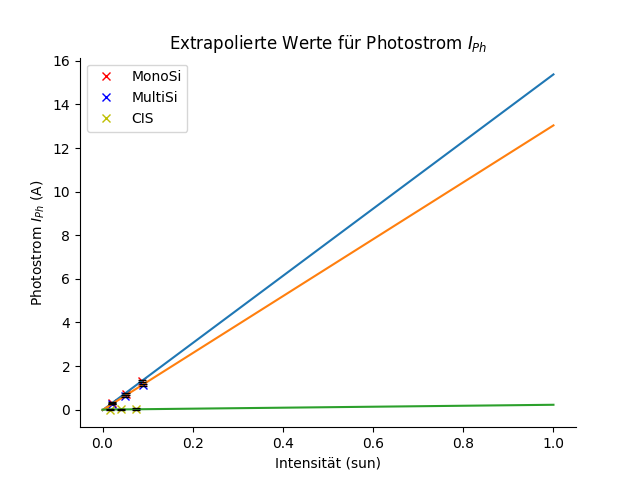
\includegraphics[width = 12cm]{Bilder/ExtrapolierteIPh.png}
\end{figure} 

Dabei ist es beeindruckend, wie gut die Daten in einen linearen Zusammenhang zu setzen sind.


\begin{figure}[ht]
    \centering
    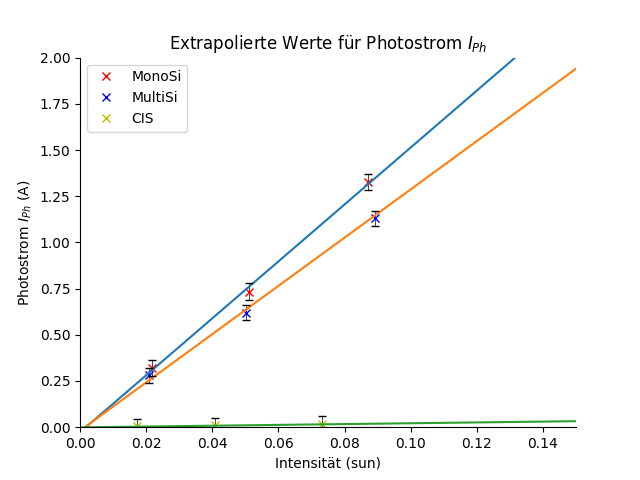
\includegraphics[width = 12cm]{Bilder/ExtrapolierteIPhAusschnitt.png}
    \caption{Ausschnitt der obigen Abbildung}
\end{figure} 
